In this section, we introduce the Codelet model based brain-inspired computing platform taking artificial neural network for example. Due to the directed connected structure of artificial neural network is very similar to that of Codelet graph, we map the components of artificial neural network to corresponding components of Codelet model.
\subsection{Neuron}
Neuron is the basic element of artificial neural network. Its operating mechanism is shown in Figure 4. It takes the outputs of the predecessor neuron as inputs, add them to the weighted sum, activate it through non-linear functions and sent the output to the subsequent neuron, which is similar to the firing mechanism of Codelet. So we model neurons as Codelets, allowing Codelet to perform different neural functions by inheriting from the Codelet class and overloading the fire() function. 
 
%\textcolor{red}{Figure 4}
\begin{figure}[h]
\caption{Figure 4}
\centering
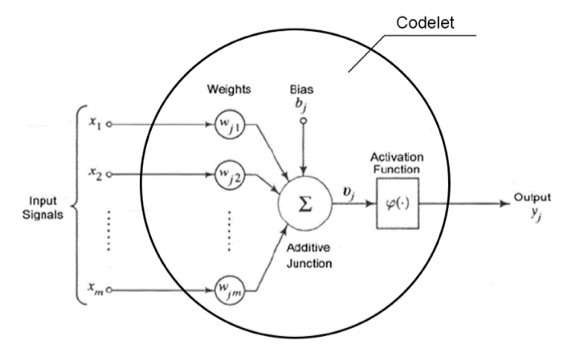
\includegraphics[width=1\textwidth]{Fig/figure4.png}
\end{figure}

Considering the overhead of Codelets executing on CUs, modeling each neuron as a Codelet will waste a lot of CPU time to switch between Codelets and reduce efficiency. On the other hand, modeling too many neurons as a Codelet loses the advantage of fine-grained parallel scheduling. After experimenting, we found that modeling 10-15 neurons as a Codelet can make the parallel computing achieve the highest efficiency.

\subsection{Layer}
Neurons in the artificial neural network are clustered into layers and neurons in the same layer perform the similar function and rely on the same input data. For some special types of neural layers, such as convolution layers, the neurons share the weights. Intuitively, the memory access time can be reduced by pre-loading shared input data or shared parameters between neurons into the cache, which is similar to the role of TP in the Codelet model. Therefore, we model the neural layer as a TP, which is inherited from the ThreadedProcedure class, and assign the corresponding local data storage area and the corresponding function's Codelet according to the type of the neural layer. Currently supported neural layer types are: convolutional layer, fully connected layer, pooling layer, Softmax classifier. An overview of layer built as TP is shown in Figure 5. The local data stores input data required by neurons, the weight parameters and the output data. Neurons only communicate with the local data, while the local data is responsible for data transmission between layers.
 
%\textcolor{red}{Figure 5}
\begin{figure}[h]
\caption{Figure 5}
\centering
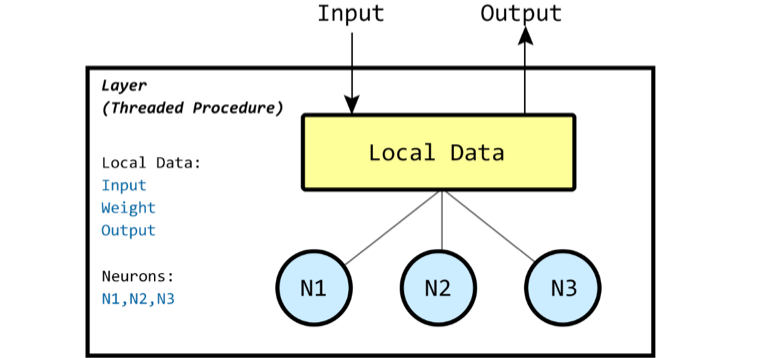
\includegraphics[width=1\textwidth]{Fig/figure5.png}
\end{figure}

\subsection{Signal/Data Transmission}
Because DARTS is based on shared address memory space, data transmission is completed by shared memory, while the signal transmission is complete by function call.
 
%\textcolor{red}{Figure 6}
\begin{figure}[h]
\caption{Figure 6}
\centering
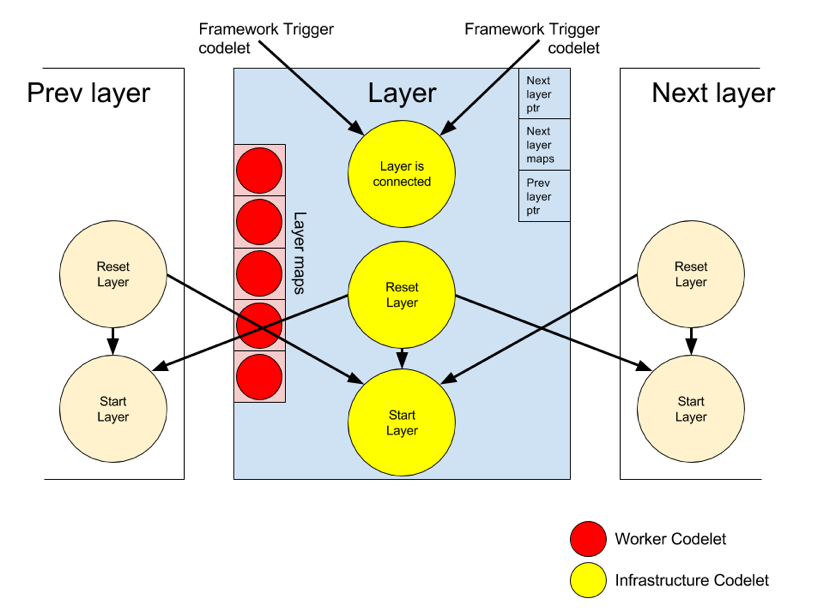
\includegraphics[width=1\textwidth]{Fig/figure6.png}
\end{figure}
Figure 6 shows the connection between a neural layer with its precursor and subsequent layer. Each layer contains the Codelets and local data. The red cells represent the working Codelet, responsible for the computation. The yellow cells represent the synchronous Codelet, responsible for the construction of the data signal transmission path between the Codelets. The local data contains relevant data, as well as the Codelet address that belong to precursor and subsequent layer which will be used for the construction of the data signal transmission path. When a layer is initialized, it will first confirm its connection with the precursor and subsequent layer via Codelet LayerIsConnected, and obtain the Codelet addresses of precursor and subsequent layer. Codelet ResetLayer and StartLayer play a role of synchronization in the pipeline execution. To avoid data racing during the pipeline execution, the layer ready to be executed and its subsequent layer should be reset. Therefore, when all the Codelets of a layer finish calculating, Codelet ResetLayer will be reset the Layer and signal Codelet StartLayer of itself, its precursor and its subsequent layer. When Codelet StartLayer collects three signals, it sets Codelets of the three layers as executable and waits to be fired by precursor Codelets.

\subsection{Construction and Execution of Neural Network}
As have introduced in Section 3.2, TP can be regarded as an asynchronous function call that provides a way to construct a CDG. Thus, we use a class Framework that calls TPs of all the layers in a network to construct a Codelet Graph that corresponding to the network. When a complete neural network framework is set up, the data flows in the framework in a pipelining manner.
In order to give full play to the advantages of asynchronous execution model, a Codelet will directly send signals to the subsequent Codelet after the completion of itself without waiting for the completion of the entire layer. Likewise, Codelet does not have to wait for the entire Codelet to start. Once all the input dependencies are satisfied, the Codelet will directly be added to the pending executed Codelet queue. In general, all Codelets are executed asynchronously and there is no specific synchronization point. 

\subsection{Multi-Framework Concurrency}
Although we have subdivided the parallel processing granularity into neuron levels, due to the structure of the neural network, the number of concurrent codelets to be executed may be less than the currently available number of computing units, i.e. the computing power is not fully utilized. For example, for the neural network shown in Figure 7, the maximum number of codelets to be executed at the same time is only 5 (the hidden layer neurons are all activated). If the computer has more than 5 computing units, the excess computing units remain idle. Therefore, we adopted a second-level parallel architecture, calling multiple frameworks simultaneously, i.e. processing multiple samples concurrently to make full use of all computing units. Since multiple frames use the same set of neural network parameters, the set of parameters should be stored in the main program and passed from the main program to each frame, as shown in Figure 8.
 
%\textcolor{red}{Figure 7}
\begin{figure}[h]
\caption{Figure 7}
\centering
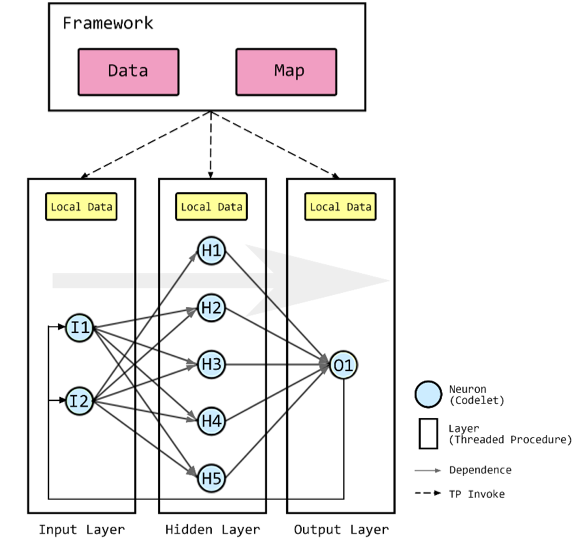
\includegraphics[width=1\textwidth]{Fig/figure7.png}
\end{figure}
 
%\textcolor{red}{Figure 8}
\begin{figure}[h]
\caption{Figure 8}
\centering
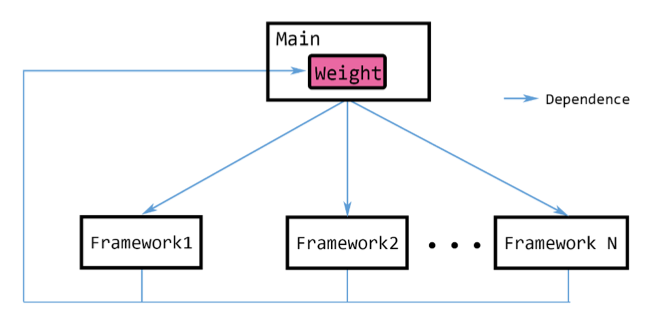
\includegraphics[width=1\textwidth]{Fig/figure8.png}
\end{figure}

\subsection{Training and Inference}
For the training of neural networks, we use batch training. Each batch of samples is distributed to all the frameworks and executed in parallel. When all the samples from a batch finish executing, the main program updates the parameters and then starts the next batch of sample training. The data flow diagram is shown in FIG. 6. For the inference of neural network, the output of each sample can be directly output without any data exchange because the inference of each sample is independent to each other.
